%% progress-report-8-SubmapVisualization+ROSPackage tex file.
%% Completed By Yuyang Rong(rongyy@shanghaitech.edu.cn) and
%% Jianxiong Cai(caijx@shanghaitech.edu.cn)
%%
%% To edit this file, please use indentions with tab size of 2.
%%

%% File name unchanged. This is just a temp file.

\documentclass[conference,compsoc]{IEEEtran}
\usepackage{cite}
\usepackage{listings}
\usepackage{blindtext}
\usepackage{enumitem}
% for coding highlight
\usepackage{graphicx}
\usepackage{subfigure}
\usepackage[colorlinks=true,urlcolor=blue]{hyperref}
\usepackage{amsmath, amsthm, amssymb}
\usepackage{subfloat}
\usepackage{ulem}
\usepackage{float}
\usepackage{indentfirst}
\newcommand{\subparagraph}{}
\begin{document}
\title{
	Computer Vision Course Project Proposal\\
	Gambody(TBD) \\
}


% author names and affiliations
% use a multiple column layout for up to three different
% affiliations
\author{
	\IEEEauthorblockN{Yuyang Rong, Jingyi Huang, Anqi Pang, Jianxiong Cai, Ziyue Li}
	\IEEEauthorblockA{
		School of Information Science and Technology \\
		ShanghaiTech University \\
	}
}

\maketitle

\begin{abstract}
	In this proposal we are going to propose our basic idea of our visual game called gambody. In this game player will have to move his body to reach certain objective. We will further explain how we are expecting this game to be, what have other people done, how we plan to implement it and how we evaluate it.
\end{abstract}
\section{Introduction}
	\par
		Nowadays there have been more and more games based on camera as an interface.
		People are more than happy to free themselves from keyboards and screens.
		Games like Pokemon Go rocketed in the summer of 2016, whose game mechanism heavily rely on AR.
		Hence, we are more than delighted and exciting when we decided to make our own game based om camera.
	\par
		We found a popular game called \textit{Hole in the Wall}. In this game one (or two) player(s) are facing a moving wall with a certain shape of hole, the player have to make certain pose to pass the moving wall or he will be pushed into the water.
		Such game is interesting but householders can never have the privilege to play in family gatherings or parties since one can hardly find a moving wall nor adequate safety measurements.
		\begin{figure}[h]
			\centering
			
\includegraphics[width=0.8\linewidth]{./Pic/HIW_Logo}
			\caption{Game Logo}
		\end{figure}
		\begin{figure}[h]
			\centering
			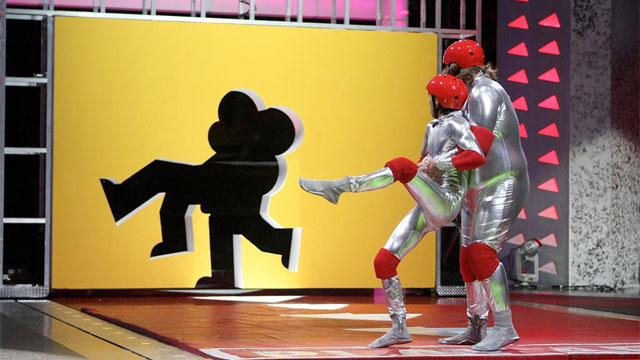
\includegraphics[width=0.45\linewidth]{./Pic/HIW_RedTeam}
			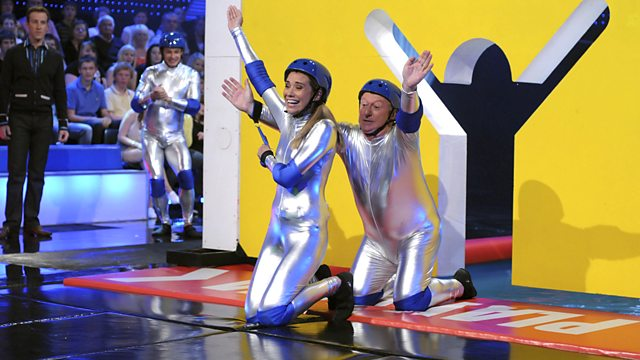
\includegraphics[width=0.45\linewidth]{./Pic/HIW_BlueTeam}
			\caption{Two players in the game posing to pass the wall.}
		\end{figure}
	\par

	\par
		To fix this, we are going to implement a system based on camera so that every one can play this game.
		In our work, we will be using camera to track real person, it will also give player a bounding box (moving wall).
		The box and player's outfit is compared by our system, the return should be a pass (True) or no pass (False).
	\par
		We will not stop here.
		A more interesting topic would be noise cancellation.
		Ideally the background should not change, but non-relevant objects (pets, non-player person, etc.) may come into the scene.
		We want our system to cancel these objects out and only sees the players so that players will not fail because their friends are behind them.
	\par
\section{Related Work}
	\par
		There are several ways to implement it.
	\par
		One is to use contour tracking algorithms \cite{panin2006efficient}, which will recognize human body's contour and keep tracking this contour. This method is of high efficiency. However, it requires user to specify curves in server frames. Some related work also uses it for Rotoscoping\cite{agarwala2004keyframe}.
	\par
		Another is to use RGB-D information to recognize human body, and this is widely used in Kinect games\cite{buys2014adaptable}.
	\par
		% TODO: Kinect game implemented last year.
		% TODO: OpenCV API
		% TODO: Real-time real-person to comic person. Bilibili poster Pangthon mentioned.
\section{Approach}
	\par
		For we are doing something related with games, so we can just tacitly approve it's an indoor scenario, cameras are usually at fixed locations. Most approach for RGB-D requires pre-processing by background subtraction and initialization poses, but we want to use RGB information only, so we prefer to using contour tracking.
	\par
		To implement this game, we need to track human body and sometimes human poses. A real-time People Finder (Pfinder) should be implemented to track the person, get the contour information, and recognize the pose and combine all the information into the game. The pipeline is listed below:
	\par
		\begin{figure}[h]
			\centering
			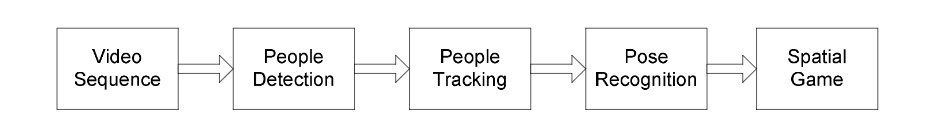
\includegraphics[width=1\linewidth]{./Pic/pipeline}
			\caption{The pipeline of such a game}
		\end{figure}
		In terms of people detection, for an indoor scenario, cameras are usually at fixed locations, motion of the scene does not exist when doing foreground object extraction. Therefore, background subtraction is a quite suitable method in this case. After that we can keep tracking human body using contour detection. Then we need to do torso and hand (if needed) segmentation, recognizing pose. Finally we combine all the things in the game.
	\par
\section{Evaluation}
	\par
		Hopefully, the results of background subtraction, contour detection and torso and hand segmentation should be robust if the number of players is predetermined. But if we continue to add support for ignoring the appearance of non-relevant objects, noise cancellation needs to be implemented robustly.
	\par
		In the end, our demo will be a somatosensory game based on camera imitating the real-world game \textit{Hole in the Wall}.

\bibliographystyle{IEEEtran}
%% De-comment this line if you have any reference.
%% And don't forget to change .bib file.
\bibliography{proposal}
\end{document}
